% ============================================================================
% Lecture 10 (B09): Automatic Differentiation for DEQNs
% Deep Learning for Solving and Estimating Dynamic Models in Economics and Finance
% Course author: Simon Scheidegger
% ============================================================================

\documentclass[aspectratio=169,11pt]{beamer}

% ---------- Theme and colors ----------
\usecolortheme{dove}
\setbeamertemplate{navigation symbols}{}
\setbeamertemplate{footline}{%
  \hfill\usebeamerfont{page number in head/foot}%
  \usebeamercolor[fg]{normal text}%
  \insertframenumber\,/\,\inserttotalframenumber\kern1em\vskip4pt}
\setbeamerfont{frametitle}{size=\huge}

% ---------- Packages ----------
\usepackage[utf8]{inputenc}
\usepackage[T1]{fontenc}
\usepackage{amsmath,amssymb,amsfonts,mathtools}
\usepackage{bm}
\usepackage{graphicx}
\usepackage{tikz}
\usetikzlibrary{shapes,arrows.meta,positioning,calc,fit,backgrounds,patterns,decorations.pathreplacing}
\usepackage{pgfplots}
\pgfplotsset{compat=1.18}
\usepackage{booktabs}
\usepackage{hyperref}
\usepackage{multicol}
\usepackage{xcolor}
\usepackage{listings}
\usepackage{tcolorbox}
\tcbuselibrary{listings,skins}

% ---------- Custom colors ----------
\definecolor{uzhblue}{rgb}{0,0,0.5}
\definecolor{uzhgreylight}{RGB}{236,238,241}
\definecolor{uzhgreydark}{RGB}{81,86,94}
\definecolor{harvardcrimson}{RGB}{153,0,0}
\definecolor{unil@blue}{RGB}{0,140,204}
\definecolor{unil@black}{RGB}{35,31,32}
\definecolor{darkgreen}{RGB}{0,100,0}
\definecolor{darkred}{RGB}{139,0,0}
\definecolor{softblue}{RGB}{70,130,180}
\definecolor{softorange}{RGB}{230,159,0}
\definecolor{softgreen}{RGB}{0,158,115}
\definecolor{codebg}{RGB}{248,248,242}
\definecolor{codekw}{RGB}{0,102,153}
\definecolor{codestr}{RGB}{153,51,0}
\definecolor{codecomm}{RGB}{0,102,0}

% ---------- Beamer colors ----------
\setbeamercolor{frametitle}{bg=uzhgreylight, fg=uzhblue}
\setbeamercolor{title}{fg=uzhblue}
\setbeamercolor{structure}{fg=uzhblue}
\setbeamercolor{block title}{bg=unil@blue, fg=white}
\setbeamercolor{block body}{bg=uzhgreylight}
\setbeamercolor{block title alerted}{bg=darkred,fg=white}
\setbeamercolor{block body alerted}{bg=red!5}
\setbeamercolor{block title example}{bg=darkgreen,fg=white}
\setbeamercolor{block body example}{bg=green!5}
\setbeamercolor{item}{fg=unil@black}
\setbeamercolor{normal text}{fg=unil@black}

% ---------- Emphasis ----------
\newcommand{\emphc}[1]{\textcolor{harvardcrimson}{#1}}
\hypersetup{colorlinks,linkcolor=harvardcrimson,urlcolor=harvardcrimson}

% ---------- Math commands ----------
\newcommand{\R}{\mathbb{R}}
\newcommand{\E}[1]{\mathbb{E}\!\left[#1\right]}
\newcommand{\Et}[1]{\mathbb{E}_t\!\left[#1\right]}
\DeclareMathOperator*{\argmin}{arg\,min}
\DeclareMathOperator*{\argmax}{arg\,max}

% ---------- Listings for Python ----------
\lstdefinestyle{py}{
  language=Python,
  basicstyle=\ttfamily\scriptsize,
  keywordstyle=\color{codekw}\bfseries,
  stringstyle=\color{codestr},
  commentstyle=\color{codecomm}\itshape,
  showstringspaces=false,
  frame=single,
  framesep=3pt,
  backgroundcolor=\color{codebg},
  rulecolor=\color{uzhgreydark!40},
  breaklines=true,
  columns=fullflexible,
  keepspaces=true,
  xleftmargin=2pt,
  xrightmargin=2pt,
}
\lstset{style=py}

% ---------- Title ----------
\title[Lecture 06 (B05)]{Lecture 06 (B05): Automatic differentiation for DEQNs}
\subtitle{From the Lagrangian primitive to two-tape Euler residuals}
\author{Simon Scheidegger}
\institute{HEC, University of Lausanne}
\date{}

\begin{document}

% ============================================================================
% PART 0: TITLE & ROADMAP
% ============================================================================

{\setbeamercolor{background canvas}{bg=uzhgreylight}
\begin{frame}
\titlepage
\vspace{-0.4cm}
\begin{center}
{\footnotesize A primer to be used alongside the autodiff notebooks (\texttt{02\_Brock\_Mirman\_AutoDiff\_DEQN}, \texttt{03\_Brock\_Mirman\_Uncertainty\_AutoDiff\_DEQN})\\
\texttt{02\_Brock\_Mirman\_AutoDiff\_DEQN} and \texttt{03\_Brock\_Mirman\_Uncertainty\_AutoDiff\_DEQN}.}\\[4pt]
{\footnotesize Materials: \url{https://github.com/sischei/Deep_Learning_for_Solving_And_Estimating_Dynamic_Economic_Models}}
\end{center}
\end{frame}
}

\begin{frame}{Roadmap}
\begin{enumerate}\itemsep4pt
  \item \textbf{Motivation.} Where do derivatives appear in our models?
  \item \textbf{Three ways to differentiate.} Symbolic, finite differences, autodiff.
  \item \textbf{How autodiff works} -- computational graph, forward vs reverse mode.
  \item \textbf{Analytical warm-ups.} CRRA utility, Cobb--Douglas, capital adjustment cost.
  \item \textbf{Brock--Mirman by hand.} Lagrangian, FOC, Bellman, envelope theorem.
  \item \textbf{Brock--Mirman by autodiff.} The one-line Euler residual; notebooks 03, 04.
  \item \textbf{Pitfalls of autodiff.} What it can (and cannot) do for you.
  \item \textbf{Takeaways.}
\end{enumerate}
\vspace{6pt}
\begin{block}{Prerequisites}
\small
A little calculus, a little Python. \emph{No prior exposure to autodiff assumed.}
\end{block}
\end{frame}

% ============================================================================
% PART 1: MOTIVATION
% ============================================================================

\section*{1. Motivation}

\begin{frame}{Derivatives are \emph{everywhere} in macro-finance}
\begin{columns}[t]
\column{0.5\textwidth}
\begin{block}{Where they show up}
\small
\begin{itemize}\itemsep3pt
  \item \emphc{First-order conditions} of optimization problems (consumer, firm, planner).
  \item The \emphc{envelope theorem} relating $V'(\cdot)$ to $\partial \mathcal{L}/\partial (\text{state})$.
  \item \emphc{Gradient descent} to train neural networks.
  \item \emphc{Sensitivity analysis / Greeks / UQ}: how does output $y$ move with input $x$?
  \item \emphc{Newton / quasi-Newton} solvers for equilibrium systems.
  \item \emphc{Implicit differentiation} for comparative statics.
\end{itemize}
\end{block}

\column{0.5\textwidth}
\begin{alertblock}{The pen-and-paper tax}
\small
Every time we write a new model we currently:
\begin{enumerate}\itemsep2pt
  \item Write the Lagrangian.
  \item Take FOCs by hand.
  \item Apply the envelope theorem by hand.
  \item Code the resulting expressions.
\end{enumerate}
Change utility function~$\Rightarrow$ redo steps~1--4.\\
Change production function~$\Rightarrow$ redo steps~1--4.\\
One typo $\Rightarrow$ wrong solver, silently.
\end{alertblock}
\end{columns}
\vspace{4pt}
\centerline{\emphc{\textbf{Goal of today:}} write the model once, let the computer do calculus.}
\end{frame}

\begin{frame}{Four reasons to care today}
\small
\begin{enumerate}\itemsep5pt
\item \textbf{FOCs of dynamic problems.} Euler equation asks for $\partial u/\partial c_t$, $\partial V/\partial K_{t+1}$. Both are derivatives of things we already coded.
\item \textbf{Envelope theorem.} $V'(K) = \partial \mathcal{L}/\partial K$ at the optimum, where $\mathcal{L}$ is the Lagrangian. Another derivative of something we already coded.
\item \textbf{Neural-network training.} $\partial \mathrm{loss}/\partial \theta$ for \emph{millions} of parameters $\theta$. Can't do this by hand.
\item \textbf{Sensitivities and uncertainty quantification.} $\partial (\text{policy})/\partial (\text{parameter})$ for robustness, comparative statics, and deep UQ (Lectures 27--29).
\end{enumerate}
\vspace{4pt}
\begin{exampleblock}{Today's punchline}
\small For \emph{all} these uses, \texttt{tf.GradientTape} (or \texttt{jax.grad}, or \texttt{torch.autograd}) replaces pages of algebra. And it is \emph{exact} -- not approximate.
\end{exampleblock}
\end{frame}

\begin{frame}{Preview: the pen-and-paper tax, visualised}
\footnotesize Notebook~01 (Brock--Mirman, the autodiff version is nb~02) needed \emph{two pages} of algebra before we could code the loss:
\begin{center}
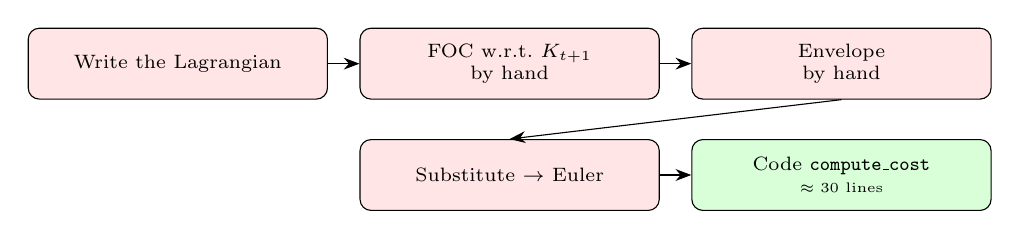
\begin{tikzpicture}[node distance=4mm]
\node[draw, fill=red!10, rounded corners, minimum width=3.8cm, minimum height=0.9cm, font=\scriptsize, align=center] (a) {Write the Lagrangian};
\node[draw, fill=red!10, rounded corners, minimum width=3.8cm, minimum height=0.9cm, font=\scriptsize, align=center, right=of a] (b) {FOC w.r.t.\ $K_{t+1}$\\by hand};
\node[draw, fill=red!10, rounded corners, minimum width=3.8cm, minimum height=0.9cm, font=\scriptsize, align=center, right=of b] (c) {Envelope\\by hand};
\node[draw, fill=red!10, rounded corners, minimum width=3.8cm, minimum height=0.9cm, font=\scriptsize, align=center, below=5mm of b] (d) {Substitute $\to$ Euler};
\node[draw, fill=green!15, rounded corners, minimum width=3.8cm, minimum height=0.9cm, font=\scriptsize, align=center, right=of d] (e) {Code \texttt{compute\_cost}\\{\tiny $\approx 30$ lines}};
\draw[-{Stealth[length=2mm]}] (a) -- (b);
\draw[-{Stealth[length=2mm]}] (b) -- (c);
\draw[-{Stealth[length=2mm]}] (c.south) -- ($(d.north)$);
\draw[-{Stealth[length=2mm]}] (d) -- (e);
\end{tikzpicture}
\end{center}
Notebook~03 (same model, autodiff) collapses all four red boxes into one function:
\begin{center}
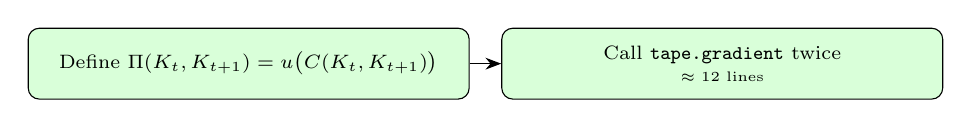
\begin{tikzpicture}[node distance=4mm]
\node[draw, fill=green!15, rounded corners, minimum width=5.6cm, minimum height=0.9cm, font=\scriptsize, align=center] (x) {Define $\Pi(K_t,K_{t+1}) = u\bigl(C(K_t,K_{t+1})\bigr)$};
\node[draw, fill=green!15, rounded corners, minimum width=5.6cm, minimum height=0.9cm, font=\scriptsize, align=center, right=of x] (y) {Call \texttt{tape.gradient} twice\\ {\tiny $\approx 12$ lines}};
\draw[-{Stealth[length=2mm]}] (x) -- (y);
\end{tikzpicture}
\end{center}
\emphc{\textbf{Everything we learn today leads to that green box on the right.}}
\end{frame}

% ============================================================================
% PART 2: THREE WAYS TO DIFFERENTIATE
% ============================================================================

\section*{2. Three ways to take a derivative}

\begin{frame}{Three ways to take a derivative}
\footnotesize
Given a function $f:\R^n \to \R$ and a point $x_0$, we can compute $\nabla f(x_0)$ in three different ways:
\vspace{3pt}
\begin{center}
\renewcommand{\arraystretch}{1.2}
\begin{tabular}{p{2.4cm} p{3.4cm} p{3.8cm} p{2.8cm}}
\toprule
& \textbf{Symbolic} & \textbf{Finite differences} & \textbf{Autodiff} \\
\midrule
\emph{Tool} & Mathematica, SymPy & a calculator, any language & PyTorch/TF/JAX \\
\emph{Accuracy} & exact & $O(h)$ or $O(h^2)$ & exact (machine $\epsilon$) \\
\emph{Cost/dim} & linear, blows up & \emphc{$n+1$ fcn evals} & \emphc{$\sim 2\times$ one eval} \\
\emph{Expr.\ swell} & yes, often bad & no & no \\
\emph{Works on code?} & limited & yes & yes \\
\emph{Step size?} & no & \emphc{yes -- hard!} & no \\
\bottomrule
\end{tabular}
\end{center}
\vspace{4pt}
\begin{itemize}\itemsep2pt
\item We briefly meet each; focus is on \emphc{finite differences} (the historical default) and \emphc{autodiff} (the modern default for ML and macro).
\end{itemize}
\end{frame}

\begin{frame}[fragile]{Method 1: symbolic differentiation}
\small \textbf{Idea:} manipulate an algebraic expression to produce a new algebraic expression.
\begin{exampleblock}{Small example}
\small
\begin{lstlisting}[language=Python,basicstyle=\ttfamily\scriptsize]
>>> from sympy import symbols, sin, log, diff
>>> x = symbols('x')
>>> f = sin(x**2) + log(1 + x**3)
>>> diff(f, x)
2*x*cos(x**2) + 3*x**2/(x**3 + 1)
\end{lstlisting}
\end{exampleblock}
\begin{columns}
\column{0.55\textwidth}
\textbf{Strengths}
\begin{itemize}\itemsep2pt
\item Exact, human-readable answer.
\item Great for \emph{one} clean formula.
\item Can reveal analytical structure (cancellations, monotonicity).
\end{itemize}
\column{0.45\textwidth}
\textbf{Weaknesses}
\begin{itemize}\itemsep2pt
\item \emphc{Expression swell}: the derivative of a product of $n$ terms has $n$ summands, each more complex than the original.
\item Cannot differentiate arbitrary \emph{code} (loops, branches).
\end{itemize}
\end{columns}
\end{frame}

\begin{frame}[fragile]{Method 2: finite differences}
\small \textbf{Idea:} approximate the derivative by the definition itself.
\[
f'(x_0) \;\approx\; \underbrace{\frac{f(x_0+h) - f(x_0)}{h}}_{\text{forward}}
\qquad\text{or}\qquad
\underbrace{\frac{f(x_0+h)-f(x_0-h)}{2h}}_{\text{central, accuracy }O(h^2)}
\]
\begin{lstlisting}[language=Python,basicstyle=\ttfamily\scriptsize]
def fd_grad(f, x, h=1e-6):
    return (f(x + h) - f(x - h)) / (2*h)
\end{lstlisting}

\textbf{Pros.} Trivial to implement; treats $f$ as a black box.\\[2pt]
\textbf{Cons.} Two sources of error fight each other:
\begin{itemize}\itemsep2pt
\item \emphc{Truncation error.} Taylor: $f(x+h) = f(x) + f'(x)h + \tfrac{1}{2}f''(x)h^2 + \ldots$; the discarded terms give error $O(h)$ (or $O(h^2)$ for central).
\item \emphc{Rounding error.} Computer stores numbers with $\sim 16$ decimal digits. Computing $f(x+h)-f(x-h)$ subtracts two nearly equal numbers $\Rightarrow$ \emph{catastrophic cancellation}; error roughly $\epsilon / h$.
\end{itemize}
\centerline{Optimal $h$ is a \emph{compromise}, and it ruins your accuracy.}
\end{frame}

\begin{frame}{Finite differences: the classic U-curve}
\footnotesize For central FD applied to $f(x) = \exp(x)$ at $x=1$:
\begin{center}
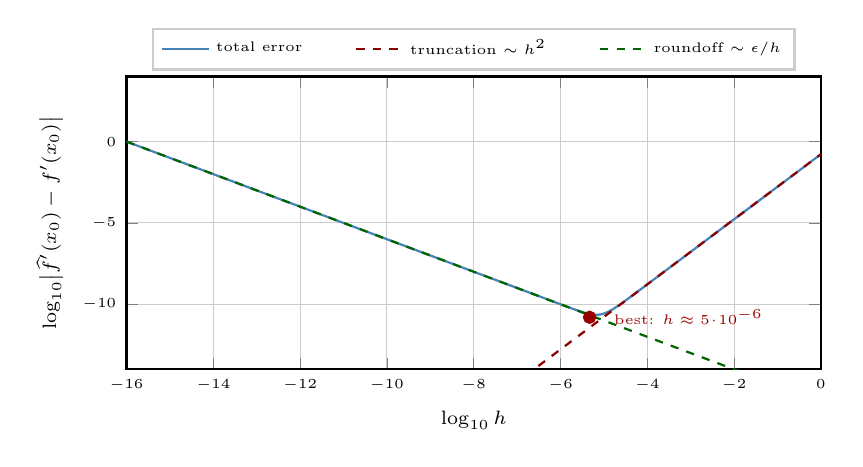
\begin{tikzpicture}
\begin{axis}[
    width=10.4cm, height=5.3cm,
    xlabel={$\log_{10} h$}, ylabel={$\log_{10}\bigl|\widehat f'(x_0) - f'(x_0)\bigr|$},
    xmin=-16, xmax=0, ymin=-14, ymax=4,
    grid=both, minor grid style={draw=black!8}, major grid style={draw=black!20},
    samples=200, thick,
    legend style={
        at={(0.5,1.02)}, anchor=south,
        legend columns=-1, font=\tiny,
        fill=white, draw=uzhgreydark!30,
        /tikz/every even column/.append style={column sep=0.6cm},
    },
    axis line style={-},
    label style={font=\scriptsize}, tick label style={font=\tiny},
]
\addplot[domain=-16:0, thick, softblue] {log10(10^(-16)/10^x + 10^(2*x)/6)};
\addplot[dashed, darkred, thick, domain=-16:0] {log10(10^(2*x)/6)};
\addplot[dashed, darkgreen, thick, domain=-16:0] {log10(10^(-16)/10^x)};
\addplot[only marks, mark=*, mark size=2pt, harvardcrimson]
    coordinates {(-5.33, -10.8)};
\node[font=\tiny, harvardcrimson, anchor=west] at (axis cs:-5.0,-10.8) {best: $h \approx 5\!\cdot\!10^{-6}$};
\legend{total error, truncation $\sim h^2$, roundoff $\sim \epsilon/h$}
\end{axis}
\end{tikzpicture}
\end{center}
\begin{itemize}\itemsep1pt
\item \emphc{Best achievable error} (1st derivative, central FD): $\sim 10^{-11}$; we \emph{lose 5--8 digits} of precision.
\item \emph{Second derivatives}: lose $\sim 10$ digits. Hessians are essentially numerical noise.
\end{itemize}
\end{frame}

\begin{frame}{Method 3: automatic differentiation -- the elevator pitch}
\small
\begin{block}{Key insight}
Every program is a composition of \emphc{elementary operations} ($+,-,\times,/,\exp,\log,\sin,\ldots$) whose derivatives we know in closed form. The chain rule mechanically combines these into the derivative of \emph{any} program.
\end{block}
\vspace{4pt}
\begin{center}
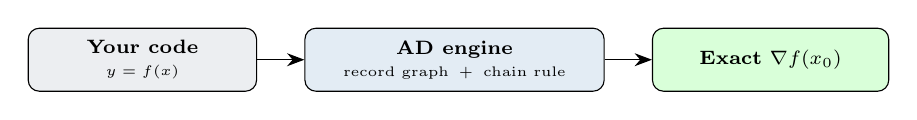
\begin{tikzpicture}[node distance=6mm]
\node[draw, fill=uzhgreylight, rounded corners, minimum width=2.9cm, minimum height=0.8cm, font=\scriptsize, align=center] (code) {\textbf{Your code}\\ {\tiny $y = f(x)$}};
\node[right=of code, draw, fill=softblue!15, rounded corners, minimum width=3.8cm, minimum height=0.8cm, font=\scriptsize, align=center] (ad) {\textbf{AD engine}\\ {\tiny $\text{record graph}\;+\;\text{chain rule}$}};
\node[right=of ad, draw, fill=green!15, rounded corners, minimum width=3.0cm, minimum height=0.8cm, font=\scriptsize, align=center] (grad) {\textbf{Exact} $\nabla f(x_0)$};
\draw[-{Stealth[length=2.2mm]}] (code) -- (ad);
\draw[-{Stealth[length=2.2mm]}] (ad) -- (grad);
\end{tikzpicture}
\end{center}
\vspace{2pt}
\begin{itemize}\itemsep3pt
\item \emphc{Exact to machine precision.} No truncation, no cancellation.
\item \emphc{Works on code}, not just formulas. If it \emph{runs}, it can be differentiated (with caveats we'll see).
\item \emphc{No step size}, no tuning.
\item \emphc{Reverse-mode cost} $\approx 2$--$4\times$ the cost of evaluating $f$, \emph{independent of dimension}.
\end{itemize}
\end{frame}

% ============================================================================
% PART 3: HOW AUTODIFF WORKS
% ============================================================================

\section*{3. How autodiff works}

\begin{frame}{Autodiff in plain English}
\small
Three statements, in order. None of them is technical.
\begin{enumerate}\itemsep4pt
\item \textbf{Every program is a chain of elementary operations.} When you compute $y = x^2 + \sin(x)$, the computer doesn't see the formula. It sees: ``square $x$, take sine of $x$, add the two''. That's three elementary steps, each with a known derivative.
\item \textbf{The chain rule composes derivatives.} If $y$ is built from $x$ via three elementary steps, then $dy/dx$ is built from those three local derivatives by the chain rule -- mechanically. We learned this in calculus class; we now ask the computer to do it.
\item \textbf{Two passes, one cost.} The computer can apply the chain rule \emph{at the same time} it evaluates $f$ (\emphc{forward mode}) or \emph{after} evaluating $f$, walking backwards (\emphc{reverse mode}). Either way, the answer is exact and the cost is a small multiple of evaluating $f$ once.
\end{enumerate}
\vspace{4pt}
\begin{block}{The whole idea}
\small Autodiff is the chain rule, applied automatically to whatever sequence of elementary operations your code happens to execute. \emph{There is no clever new mathematics.} Just bookkeeping.
\end{block}
\end{frame}

\begin{frame}{Where do the local derivatives come from? A tiny built-in table}
\footnotesize
\textbf{Punchline.} The computer doesn't ``know calculus''. It knows a short \emphc{hardcoded table} of derivatives for \emph{elementary} operations. Every program is built from these; the chain rule composes the pieces.
\vspace{4pt}
\begin{center}
\renewcommand{\arraystretch}{1.15}
\begin{tabular}{p{3.0cm} p{3.0cm} p{5.8cm}}
\toprule
\textbf{Primitive} & \textbf{Rule (built into the framework)} & \textbf{Where written} \\
\midrule
$y = x + z$ & $\partial y/\partial x = 1,\; \partial y/\partial z = 1$ & \texttt{tf.math.add.gradient} \\
$y = x \cdot z$ & $\partial y/\partial x = z,\; \partial y/\partial z = x$ & \texttt{tf.math.multiply.gradient} \\
$y = x^{\alpha}$ & $\partial y/\partial x = \alpha x^{\alpha-1}$ & \texttt{tf.math.pow.gradient} \\
$y = \exp(x)$ & $\partial y/\partial x = \exp(x)$ & \texttt{tf.math.exp.gradient} \\
$y = \log(x)$ & $\partial y/\partial x = 1/x$ & \texttt{tf.math.log.gradient} \\
$y = \sin(x)$ & $\partial y/\partial x = \cos(x)$ & \texttt{tf.math.sin.gradient} \\
$y = \cos(x)$ & $\partial y/\partial x = -\sin(x)$ & \texttt{tf.math.cos.gradient} \\
$y = \mathrm{ReLU}(x)$ & $\partial y/\partial x = \mathbf{1}\{x > 0\}$ & \texttt{tf.nn.relu.gradient} \\
\bottomrule
\end{tabular}
\end{center}
\vspace{4pt}
That's the whole trick. TensorFlow (and PyTorch, and JAX) ship with a few hundred of these rules. Your code composes them; the chain rule composes their derivatives.
\vspace{4pt}
\begin{exampleblock}{In one sentence}
\footnotesize The computer ``knows'' $d(\sin x)/dx = \cos x$ because \emph{someone typed that rule into the framework}. We compose rules; we never re-derive them.
\end{exampleblock}
\end{frame}

\begin{frame}{Why the chain rule is enough: a 30-second worked example}
\scriptsize
Compute $\dfrac{dy}{dx}$ for $y = x^2 + \sin(x)$ at $x=2$, \emph{one elementary step at a time}.

\vspace{2pt}
\textbf{Decomposition.}  Two intermediate variables, one per elementary operation on $x$:
\[
v_1 \,:=\, x^2, \qquad v_2 \,:=\, \sin(x), \qquad y \,=\, v_1 + v_2.
\]

\vspace{2pt}
\begin{tabular}{@{}p{1.0cm}p{5.6cm}p{5.0cm}@{}}
\toprule
\textbf{Step} & \textbf{Elementary operation} & \textbf{Local derivative} \\
\midrule
\textcolor{harvardcrimson}{(1)} & $v_1 = x^2$;\; $x=2 \Rightarrow v_1 = 4$ & $\partial v_1/\partial x = 2x = 4$ \\
\textcolor{harvardcrimson}{(2)} & $v_2 = \sin(x)$;\; $x=2 \Rightarrow v_2 \approx 0.909$ & $\partial v_2/\partial x = \cos(x) \approx -0.416$ \\
\textcolor{harvardcrimson}{(3)} & $y = v_1 + v_2 \approx 4.909$ & $\partial y / \partial v_1 = 1$, \; $\partial y / \partial v_2 = 1$ \\
\bottomrule
\end{tabular}

\vspace{3pt}
\textbf{Chain rule:} $\;\dfrac{dy}{dx} = \dfrac{\partial y}{\partial v_1}\dfrac{\partial v_1}{\partial x} + \dfrac{\partial y}{\partial v_2}\dfrac{\partial v_2}{\partial x} = 1\cdot 4 + 1\cdot (-0.416) = 3.584.$

\textbf{Cross-check:} $f'(x) = 2x + \cos(x)$, so $f'(2) = 4 + \cos(2) \approx 3.584$.\;\emphc{Same answer.}

\vspace{2pt}
\emphc{Take-away.} No new mathematics, just bookkeeping along the chain.  Next: picture it as a graph; then forward vs.\ reverse mode.
\end{frame}

\begin{frame}{Same example, drawn as a computational graph}
\footnotesize The three elementary operations from the previous slide, as a directed graph:\\
\emph{nodes} = operations, \emph{arrows} = intermediate values.
\vspace{1pt}
\[
y = f(x) = x^2 + \sin(x) \quad\text{at}\quad x = 2.
\]
\vspace{-6pt}
\begin{center}
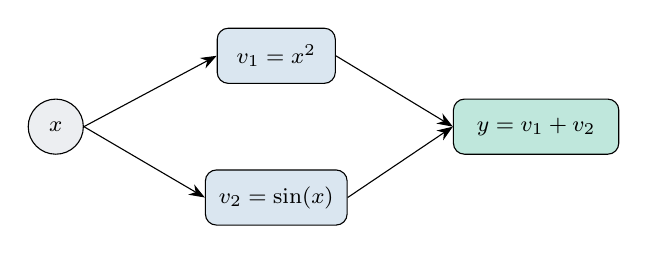
\begin{tikzpicture}[every node/.style={font=\footnotesize}]
\node[draw, circle, fill=uzhgreylight, minimum size=7mm, inner sep=0pt] (x)  at (0,0)   {$x$};
\node[draw, rounded corners, fill=softblue!20, minimum width=1.5cm, minimum height=7mm, inner sep=2pt] (v1) at (2.8, 0.9) {$v_1 = x^2$};
\node[draw, rounded corners, fill=softblue!20, minimum width=1.8cm, minimum height=7mm, inner sep=2pt] (v2) at (2.8,-0.9) {$v_2 = \sin(x)$};
\node[draw, rounded corners, fill=softgreen!25, minimum width=2.1cm, minimum height=7mm, inner sep=2pt] (y)  at (6.1, 0) {$y = v_1 + v_2$};
\draw[-{Stealth[length=2mm]}] (x.east) -- (v1.west);
\draw[-{Stealth[length=2mm]}] (x.east) -- (v2.west);
\draw[-{Stealth[length=2mm]}] (v1.east) -- (y.west);
\draw[-{Stealth[length=2mm]}] (v2.east) -- (y.west);
\end{tikzpicture}
\end{center}
\vspace{-4pt}
\begin{itemize}\itemsep1pt
\item \emphc{Nodes}: the same three elementary operations as in the table.
\item \emphc{Arrows}: intermediate values $v_1, v_2$ flowing between operations.
\item \emphc{Local derivatives live on the arrows}: $\partial v_1/\partial x = 2x$, $\partial v_2/\partial x = \cos(x)$, $\partial y/\partial v_i = 1$.
\end{itemize}
The graph is a \emph{visual organiser} for the chain rule -- and lets us state \emph{forward} and \emph{reverse} mode cleanly on the next slides.
\end{frame}

\begin{frame}{The graph carries the local derivatives -- both modes use them}
\footnotesize Same graph, annotated with each edge's local derivative:
\begin{center}
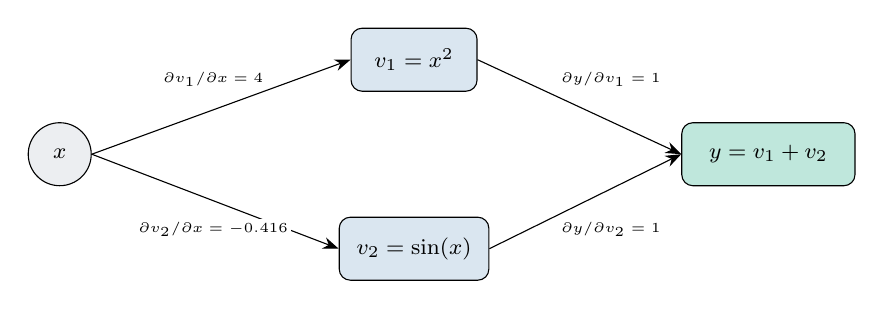
\begin{tikzpicture}[every node/.style={font=\footnotesize}]
\node[draw, circle, fill=uzhgreylight, minimum size=8mm, inner sep=0pt] (x)  at (0,0)   {$x$};
\node[draw, rounded corners, fill=softblue!20, minimum width=1.6cm, minimum height=8mm, inner sep=2pt] (v1) at (4.5, 1.2) {$v_1 = x^2$};
\node[draw, rounded corners, fill=softblue!20, minimum width=1.9cm, minimum height=8mm, inner sep=2pt] (v2) at (4.5,-1.2) {$v_2 = \sin(x)$};
\node[draw, rounded corners, fill=softgreen!25, minimum width=2.2cm, minimum height=8mm, inner sep=2pt] (y)  at (9.0, 0) {$y = v_1 + v_2$};
\draw[-{Stealth[length=2mm]}] (x.east) -- (v1.west);
\draw[-{Stealth[length=2mm]}] (x.east) -- (v2.west);
\draw[-{Stealth[length=2mm]}] (v1.east) -- (y.west);
\draw[-{Stealth[length=2mm]}] (v2.east) -- (y.west);
% Edge labels with white background
\node[font=\tiny, fill=white, inner sep=1pt] at (1.95, 0.95) {$\partial v_1/\partial x = 4$};
\node[font=\tiny, fill=white, inner sep=1pt] at (1.95,-0.95) {$\partial v_2/\partial x = -0.416$};
\node[font=\tiny, fill=white, inner sep=1pt] at (7.0, 0.95) {$\partial y/\partial v_1 = 1$};
\node[font=\tiny, fill=white, inner sep=1pt] at (7.0,-0.95) {$\partial y/\partial v_2 = 1$};
\end{tikzpicture}
\end{center}
\textbf{Two strategies for combining the edges into $dy/dx$.}
\begin{itemize}\itemsep1pt
\item \emphc{Forward mode}: walk \emph{left to right} (with $f$); accumulate $\dot v = \partial v/\partial x$ from parent $\dot u$. Read $\dot y$.
\item \emphc{Reverse mode}: walk \emph{right to left} (after $f$); accumulate $\bar v = \partial y/\partial v$ from child $\bar w$. Read $\bar x$.
\end{itemize}
Both give the same number; they differ in \emph{when} bookkeeping happens and \emph{which dimension} they scale with -- detailed next.
\end{frame}

\begin{frame}{Forward mode: propagate derivatives \emph{with} the computation}
\footnotesize
\textbf{Big idea.} Carry a \emphc{derivative tag} $\dot v$ next to every value $v$, and update both in the same forward pass.
\begin{block}{The chain rule, applied locally to each elementary operation}
\footnotesize
\[
v = g(u) \;\Rightarrow\; \dot v = g'(u)\,\dot u, \qquad
v = g(u_1,u_2) \;\Rightarrow\; \dot v = g_1\,\dot u_1 + g_2\,\dot u_2.
\]
\end{block}
\textbf{Recipe.}
\begin{enumerate}\itemsep1pt
\item Replace each $v$ in the program by the pair $(v, \dot v)$ (a \emphc{dual number}).
\item Seed at the input: $\dot x = 1$.
\item Run forward: each operation updates both the value and its tag.
\item Read $\dot y$ at the output -- this is $dy/dx$, exact.
\end{enumerate}
\emphc{Why ``forward''?} The derivative moves \emph{with} the program. \emphc{Why correct?} The chain rule, applied at every node. Next slide: in action on $y = x^2 + \sin(x)$.
\end{frame}

\begin{frame}{Forward mode: worked example on $y = x^2 + \sin(x)$ at $x=2$}
\footnotesize
\textbf{Seed} at the input: $(x,\;\dot x) = (2,\;1)$. Each elementary operation updates both fields via the chain rule:
\begin{itemize}\itemsep1pt
\item $v_1 = x^2 \Rightarrow \dot v_1 = 2x\,\dot x = 4$. So $(v_1,\dot v_1) = (4,\,4)$.
\item $v_2 = \sin(x) \Rightarrow \dot v_2 = \cos(x)\,\dot x \approx -0.416$. So $(v_2,\dot v_2) = (0.909,\,-0.416)$.
\item $y = v_1 + v_2 \Rightarrow \dot y = \dot v_1 + \dot v_2 = 3.584$.
\end{itemize}
\begin{center}
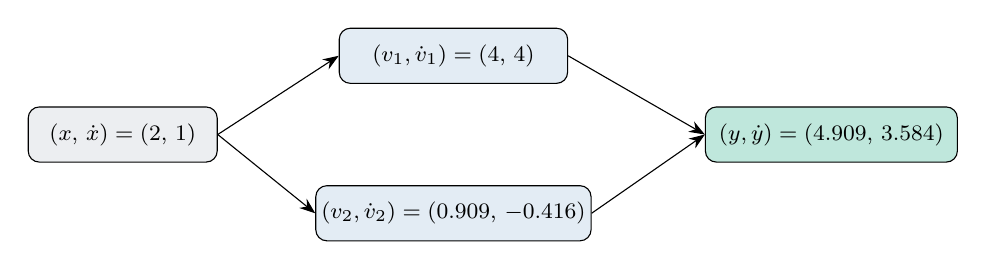
\begin{tikzpicture}[every node/.style={font=\footnotesize}]
\node[draw, rounded corners, fill=uzhgreylight, minimum width=2.4cm, minimum height=7mm, inner sep=2pt] (x)  at (0,0)   {$(x,\,\dot x) = (2,\,1)$};
\node[draw, rounded corners, fill=softblue!15, minimum width=2.9cm, minimum height=7mm, inner sep=2pt] (v1) at (4.2, 1.0) {$(v_1,\dot v_1) = (4,\,4)$};
\node[draw, rounded corners, fill=softblue!15, minimum width=3.4cm, minimum height=7mm, inner sep=2pt] (v2) at (4.2,-1.0) {$(v_2,\dot v_2) = (0.909,\,-0.416)$};
\node[draw, rounded corners, fill=softgreen!25, minimum width=3.2cm, minimum height=7mm, inner sep=2pt] (y)  at (9.0, 0) {$(y,\dot y) = (4.909,\,3.584)$};
\draw[-{Stealth[length=2mm]}] (x.east) -- (v1.west);
\draw[-{Stealth[length=2mm]}] (x.east) -- (v2.west);
\draw[-{Stealth[length=2mm]}] (v1.east) -- (y.west);
\draw[-{Stealth[length=2mm]}] (v2.east) -- (y.west);
\end{tikzpicture}
\end{center}
\textbf{Read out} $\dot y = dy/dx = 3.584$. Cross-check: $f'(2) = 4 + \cos(2) = 3.584$. \emphc{Exact.}
\begin{itemize}\itemsep1pt
\item \emphc{Cost:} $\sim 2\times$ one call to $f$.
\item \emphc{Scales with \#inputs:} for $\nabla f$ with $f:\R^n\to\R$, need $n$ forward passes. Bad for neural nets; \emph{reverse mode} (next) fixes this.
\end{itemize}
\end{frame}

\begin{frame}{Reverse mode (= backprop): propagate \emph{backwards}}
\footnotesize
\textbf{Idea.} First evaluate $f$ forward and \emph{remember} the graph. Then walk backwards, carrying the sensitivity $\bar v = \partial y / \partial v$ along each edge. Seed $\bar y = 1$ at the output.
\begin{center}
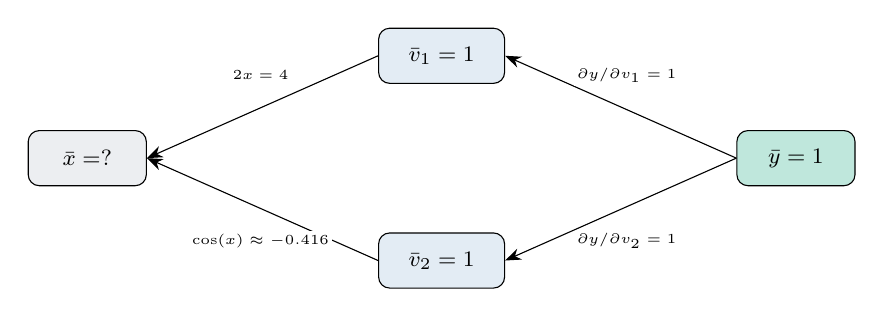
\begin{tikzpicture}[every node/.style={font=\footnotesize}]
\node[draw, rounded corners, fill=uzhgreylight, minimum width=1.5cm, minimum height=7mm, inner sep=2pt] (x)  at (0,0)   {$\bar x = ?$};
\node[draw, rounded corners, fill=softblue!15, minimum width=1.6cm, minimum height=7mm, inner sep=2pt] (v1) at (4.5, 1.3) {$\bar v_1 = 1$};
\node[draw, rounded corners, fill=softblue!15, minimum width=1.6cm, minimum height=7mm, inner sep=2pt] (v2) at (4.5,-1.3) {$\bar v_2 = 1$};
\node[draw, rounded corners, fill=softgreen!25, minimum width=1.5cm, minimum height=7mm, inner sep=2pt] (y)  at (9.0, 0) {$\bar y = 1$};
\draw[-{Stealth[length=2mm]}] (y.west) -- (v1.east);
\draw[-{Stealth[length=2mm]}] (y.west) -- (v2.east);
\draw[-{Stealth[length=2mm]}] (v1.west) -- (x.east);
\draw[-{Stealth[length=2mm]}] (v2.west) -- (x.east);
\node[font=\tiny, fill=white, inner sep=1pt] at (6.85, 1.05) {$\partial y/\partial v_1 = 1$};
\node[font=\tiny, fill=white, inner sep=1pt] at (6.85,-1.05) {$\partial y/\partial v_2 = 1$};
\node[font=\tiny, fill=white, inner sep=1pt] at (2.20, 1.05) {$2x = 4$};
\node[font=\tiny, fill=white, inner sep=1pt] at (2.20,-1.05) {$\cos(x) \approx -0.416$};
\end{tikzpicture}
\end{center}
\textbf{Rule.} $\bar x = \sum_{i:\,x\to v_i} \bar v_i \cdot \tfrac{\partial v_i}{\partial x}$. So
\[
\bar x = \bar v_1 \cdot 4 + \bar v_2 \cdot (-0.416) = 1\cdot 4 + 1\cdot(-0.416) = 3.584.
\]
\vspace{-6pt}
\begin{itemize}\itemsep1pt
\item \emphc{Cost:} $\sim 2$--$4\,T_f$; memory $\propto$ graph size (one issue we'll revisit).
\item \emphc{Scales with \#outputs:} one reverse pass per output -- great for scalar losses with many inputs.
\item \textbf{This is what TF/PyTorch/JAX do under the hood for neural nets.}
\end{itemize}
\end{frame}

\begin{frame}{Which mode to use?}
\footnotesize
For $f:\R^n \to \R^m$; $T_f$ = cost of one forward evaluation of $f$.
\vspace{2pt}
\begin{center}
\renewcommand{\arraystretch}{1.1}
\begin{tabular}{p{3.4cm} p{3.0cm} p{3.0cm} p{2.4cm}}
\toprule
\textbf{Setting} & \textbf{Dimensions} & \textbf{Mode of choice} & \textbf{Cost (full Jac.)} \\
\midrule
Neural-net training & $n\!\sim\!10^6$, $m\!=\!1$ & \emphc{Reverse} (backprop) & $2\text{--}4\,T_f$ \\
Sensitivity, many inputs $\to$ one output & $n$ large, $m\!=\!1$ & Reverse & $2\text{--}4\,T_f$ \\
Tangents, ODE solvers & $n\!=\!1$, $m$ large & \emphc{Forward} & $\sim 2\,T_f$ \\
Square Jacobian & $n = m$ & Either works & $\sim n\,T_f$ \\
\bottomrule
\end{tabular}
\end{center}
\vspace{2pt}
\begin{block}{For DEQNs (and most of this course)}
\footnotesize
Scalar loss, $n\sim 10^3$ to $10^5$ parameters. \emphc{Reverse mode wins}: one pass at $\sim 4\,T_f$ gives the gradient w.r.t.\ \emph{all} $n$ parameters. Frameworks (\texttt{tf.GradientTape}, \texttt{torch.autograd}, \texttt{jax.grad}) default to reverse mode.
\end{block}
\end{frame}

% ============================================================================
% PART 4: ANALYTICAL WARM-UPS
% ============================================================================

\section*{4. Analytical warm-ups}

\begin{frame}[fragile]{Warm-up 1: CRRA marginal utility}
\footnotesize Isoelastic (CRRA) utility with $\gamma = 2$:
\[
u(c) = \frac{c^{1-\gamma}}{1-\gamma} = -\frac{1}{c}, \quad u'(c) = c^{-\gamma} = \frac{1}{c^2}, \quad u''(c) = -\gamma c^{-\gamma-1}.
\]
\begin{lstlisting}[language=Python,basicstyle=\ttfamily\scriptsize]
import tensorflow as tf
gamma = 2.0
def u(c):                         # one-liner, model primitive
    return c**(1.0 - gamma) / (1.0 - gamma)

c = tf.Variable(3.0)
with tf.GradientTape(persistent=True) as tape:
    y = u(c)
    up = tape.gradient(y, c)      # first derivative via AD
upp = tape.gradient(up, c)        # second derivative via AD
# hand: u'(3)  = 1/9   = 0.1111...   u''(3) = -2/27 = -0.07407...
\end{lstlisting}
\begin{exampleblock}{Result}
\footnotesize AD returns $u'(3) \approx 0.11111111$ and $u''(3) \approx -0.07407407$ to machine precision. \textbf{No hand derivation.} Change $\gamma$ to $4$: the code is unchanged.
\end{exampleblock}
\end{frame}

\begin{frame}[fragile]{Warm-up 2: Cobb--Douglas marginal products}
\small Production function with $\alpha = 0.36$:
\[
f(K,L) = K^\alpha L^{1-\alpha}, \qquad
\partial_K f = \alpha\,K^{\alpha-1} L^{1-\alpha}, \qquad
\partial_L f = (1-\alpha)\,K^\alpha L^{-\alpha}.
\]
\begin{lstlisting}[language=Python,basicstyle=\ttfamily\scriptsize]
alpha = 0.36
def f(K, L):                      # model primitive
    return K**alpha * L**(1.0 - alpha)

K, L = tf.Variable(5.0), tf.Variable(2.0)
with tf.GradientTape() as tape:
    y = f(K, L)
grads = tape.gradient(y, [K, L])  # returns a list with both partials

# hand: f_K(5,2) = 0.36 * 5^(-0.64) * 2^(0.64)  ~  0.1832
#       f_L(5,2) = 0.64 * 5^(0.36) * 2^(-0.36)  ~  1.0461
\end{lstlisting}
\vspace{-2pt}
\begin{exampleblock}{Take-away}
\small One \emph{tape}, one call, \emph{both} partial derivatives. Replace Cobb--Douglas by CES: change the \texttt{def f(...)} line; \emph{the gradient line is unchanged}.
\end{exampleblock}
\end{frame}

\begin{frame}[fragile]{Warm-up 3: capital adjustment cost (by hand is annoying)}
\small Convex adjustment cost, from the IRBC model:
\[
\Gamma(K, K') \;=\; \frac{\kappa}{2}\, K \left(\frac{K'}{K} - 1\right)^2.
\]
By hand, \textbf{two partial derivatives}, each needing the \emph{quotient} and \emph{chain} rules:
\begin{align*}
\tfrac{\partial \Gamma}{\partial K'} &= \kappa\,K\,\left(\tfrac{K'}{K}-1\right)\cdot \tfrac{1}{K} \;=\; \kappa\,\left(\tfrac{K'}{K}-1\right),\\
\tfrac{\partial \Gamma}{\partial K} &= \tfrac{\kappa}{2}\,\left(\tfrac{K'}{K}-1\right)^2
 + \kappa\,K\,\left(\tfrac{K'}{K}-1\right)\cdot\left(-\tfrac{K'}{K^2}\right)\\
 &= \tfrac{\kappa}{2}\left(\tfrac{K'}{K}-1\right)^2 - \kappa\,\tfrac{K'}{K}\left(\tfrac{K'}{K}-1\right).
\end{align*}
This is the kind of algebra where \emph{typos} live.
\end{frame}

\begin{frame}[fragile]{Warm-up 3 (cont.): by autodiff}
\small
\begin{lstlisting}[language=Python,basicstyle=\ttfamily\scriptsize]
kappa = 0.3
def Gamma(K, Kp):                 # model primitive -- ONE line
    return 0.5 * kappa * K * (Kp / K - 1.0)**2

K  = tf.Variable(5.0)
Kp = tf.Variable(5.6)
with tf.GradientTape() as tape:
    g = Gamma(K, Kp)
dK, dKp = tape.gradient(g, [K, Kp])
#  AD:  dK   ~  -0.0252  (matches hand)
#       dKp  ~   0.036   (matches hand)
\end{lstlisting}
\vspace{-2pt}
\begin{block}{Observation}
\small
\textbf{Hand:} two paragraphs of algebra, one chance to typo a sign. \\
\textbf{AD:} one Python definition, \emph{zero} chances to typo. Same answer to machine precision.
\end{block}
\centerline{\emphc{This is the small version of what happens on the full Brock--Mirman Lagrangian next.}}
\end{frame}

\begin{frame}{What we've learned about AD so far}
\small
\begin{enumerate}\itemsep4pt
\item \textbf{You write only the model primitive} -- the utility function, the production function, the cost function, the Lagrangian. \emph{Not} any derivative.
\item \textbf{AD returns the derivative to machine precision}, not an approximation.
\item \textbf{Adding a new partial derivative is free} (one more entry in the argument list of \texttt{tape.gradient}).
\item \textbf{Changing the functional form leaves the gradient code untouched.}
\item \textbf{Reverse mode is cheap}: $\sim 2\text{--}4\times$ the forward pass, independent of the number of inputs.
\end{enumerate}
\vspace{8pt}
\begin{exampleblock}{Coming up}
\small Now we will apply this \emph{exactly the same pattern} to the Brock--Mirman planner's problem. First: derive the Euler equation by hand, to see what we are replacing.
\end{exampleblock}
\end{frame}

% ============================================================================
% PART 5: BROCK-MIRMAN BY HAND
% ============================================================================

\section*{5. Brock--Mirman by hand}

\begin{frame}{The deterministic Brock--Mirman model}
\small The social planner solves
\[
\max_{\{C_t, K_{t+1}\}_{t \ge 0}} \;\sum_{t=0}^{\infty} \beta^t \ln(C_t)
\quad\text{s.t.}\quad
K_{t+1} + C_t \;=\; K_t^{\alpha} + (1-\delta)\,K_t, \quad K_0\text{ given}.
\]
\vspace{-6pt}
\begin{columns}[t]
\column{0.48\textwidth}
\begin{block}{Primitives}
\small
\begin{itemize}\itemsep2pt
\item Utility: $u(C) = \ln C$.
\item Production: $Y_t = K_t^\alpha$ (Cobb--Douglas, $\alpha \in (0,1)$).
\item Depreciation rate: $\delta \in [0,1]$.
\item Discount factor: $\beta \in (0,1)$.
\end{itemize}
\end{block}
\column{0.48\textwidth}
\begin{block}{What we want}
\small
A \emph{policy function}
\[
K_{t+1} = g(K_t)
\]
that maximises lifetime utility. With $\delta = 1$ the answer is known:
\[
g(K) = \alpha\beta\, K^\alpha.
\]
We will \emph{derive} the Euler equation that $g$ must satisfy.
\end{block}
\end{columns}
\end{frame}

\begin{frame}{The sequence-form Lagrangian}
\small Attach a multiplier $\beta^t \lambda_t$ to the resource constraint at every date:
\begin{block}{Lagrangian (written out in full)}
\small
\[
\mathcal{L} \;=\; \sum_{t=0}^{\infty} \beta^t \Bigl[\, \underbrace{\ln C_t}_{\text{utility}} \;+\; \lambda_t\,\bigl(\underbrace{K_t^\alpha + (1-\delta)K_t}_{\text{resources}} \;-\; C_t \;-\; K_{t+1}\bigr)\,\Bigr].
\]
\end{block}
\vspace{2pt}
\emph{Choice variables} at each date: $C_t$ and $K_{t+1}$.\\
\emph{State} at date $t$: $K_t$, coming in from the previous period.\\[6pt]
\textbf{Plan.} Take FOCs with respect to each choice variable, combine with the constraint, and get a single difference equation in $K_t$.
\end{frame}

\begin{frame}{FOC with respect to $C_t$}
\small Differentiate $\mathcal{L}$ with respect to $C_t$ (which appears only in the $t$-th summand):
\begin{align*}
\frac{\partial \mathcal{L}}{\partial C_t} \;&=\; \beta^t \left[\frac{1}{C_t} \;-\; \lambda_t\right] \;=\; 0 \\[4pt]
\Longrightarrow\; \lambda_t \;&=\; \frac{1}{C_t} \;=\; u'(C_t).
\end{align*}
\begin{block}{Interpretation}
\small
The multiplier $\lambda_t$ equals the \emph{marginal utility of consumption}. Unsurprising -- the planner is willing to pay $u'(C_t)$ additional units of resources to get one more unit of consumption today.
\end{block}
\end{frame}

\begin{frame}{FOC with respect to $K_{t+1}$}
\small $K_{t+1}$ appears \emph{twice} in the Lagrangian: as the choice at date $t$ (with coefficient $-\beta^t \lambda_t$) and as the state at date $t+1$ (inside $K_{t+1}^\alpha + (1-\delta)K_{t+1}$, with coefficient $+\beta^{t+1}\lambda_{t+1}$).
\begin{align*}
\frac{\partial \mathcal{L}}{\partial K_{t+1}}
&= -\beta^t \lambda_t \;+\; \beta^{t+1}\,\lambda_{t+1}\,\left[\alpha K_{t+1}^{\alpha-1} + (1-\delta)\right] \;=\; 0 \\[4pt]
\Longrightarrow\; \lambda_t &= \beta\,\lambda_{t+1}\,\Bigl[\,\underbrace{\alpha K_{t+1}^{\alpha-1}}_{\text{MPK}_{t+1}} + 1 - \delta\,\Bigr].
\end{align*}
\begin{block}{Interpretation}
\small
One unit \emph{not} consumed today (costing $\lambda_t$ units of utility) becomes capital tomorrow, earning the gross rental $\mathrm{MPK}_{t+1} + 1-\delta$ in resource units, which is then valued at tomorrow's multiplier $\beta\lambda_{t+1}$.
\end{block}
\end{frame}

\begin{frame}{Combine: the Euler equation}
\small Substitute $\lambda_t = u'(C_t) = 1/C_t$ from the first FOC into the second:
\begin{block}{Euler equation (deterministic)}
\[
\frac{1}{C_t} \;=\; \beta\,\frac{1}{C_{t+1}}\,\left[\alpha K_{t+1}^{\alpha-1} + 1 - \delta\right].
\]
\end{block}
\vspace{6pt}
Equivalently, writing $r_{t+1} = \alpha K_{t+1}^{\alpha-1}$,
\[
u'(C_t) \;=\; \beta\, u'(C_{t+1}) \,(\,1 - \delta + r_{t+1}\,).
\]
\vspace{2pt}
\begin{itemize}\itemsep2pt
\item This is the \emph{consumption smoothing} condition. Marginal utility today = discounted, rate-adjusted marginal utility tomorrow.
\item This is the equation that \texttt{compute\_cost} in notebook~01 minimises the squared residual of.
\end{itemize}
\end{frame}

\begin{frame}{Recursive (Bellman) form and the envelope theorem}
\footnotesize The same problem has a recursive representation:
\[
V(K) \;=\; \max_{K'}\; \Bigl\{\, u\!\bigl(\underbrace{K^\alpha + (1-\delta)K - K'}_{= C(K,K')}\bigr) + \beta\, V(K') \,\Bigr\}.
\]
Let $g(K)$ be the optimal $K'$.\\[2pt]
\textbf{Envelope theorem.} Differentiate $V$, use the FOC $-u'(C) + \beta V'(g(K)) = 0$ to cancel terms:
\begin{align*}
V'(K) &= u'\!(C)\cdot\underbrace{[\alpha K^{\alpha-1} + 1 - \delta]}_{\partial C / \partial K} + \bigl[-u'(C) + \beta V'(g(K))\bigr]\cdot g'(K)\\
&= u'(C)\,[\alpha K^{\alpha-1} + 1 - \delta]. \qquad\text{(FOC kills the second bracket.)}
\end{align*}
\begin{alertblock}{Envelope formula}
\footnotesize
\[
V'(K_t) \;=\; u'(C_t)\,\bigl[\alpha K_t^{\alpha-1} + 1 - \delta\bigr].
\]
\emph{The derivative of $V$ equals the partial of the Lagrangian w.r.t.\ the state} -- about to be exploited.
\end{alertblock}
\end{frame}

\begin{frame}{Recap: what we derived by hand}
\small
\begin{center}
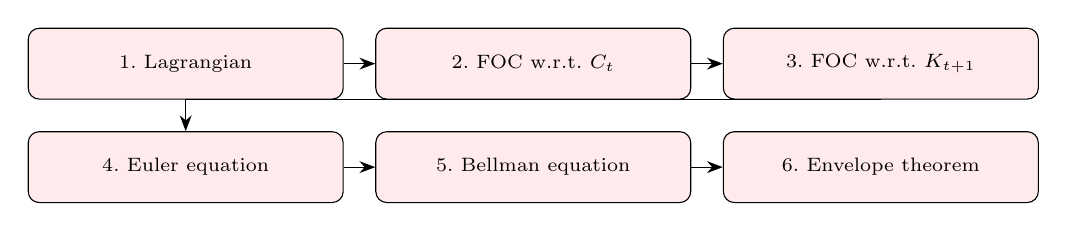
\begin{tikzpicture}[node distance=4mm, every node/.style={font=\scriptsize}]
\node[draw, rounded corners, fill=red!8, align=center, minimum width=4.0cm, minimum height=0.9cm] (a) {1.\ Lagrangian};
\node[draw, rounded corners, fill=red!8, align=center, right=of a, minimum width=4.0cm, minimum height=0.9cm] (b) {2.\ FOC w.r.t.\ $C_t$};
\node[draw, rounded corners, fill=red!8, align=center, right=of b, minimum width=4.0cm, minimum height=0.9cm] (c) {3.\ FOC w.r.t.\ $K_{t+1}$};
\node[draw, rounded corners, fill=red!8, align=center, below=of a, minimum width=4.0cm, minimum height=0.9cm] (d) {4.\ Euler equation};
\node[draw, rounded corners, fill=red!8, align=center, right=of d, minimum width=4.0cm, minimum height=0.9cm] (e) {5.\ Bellman equation};
\node[draw, rounded corners, fill=red!8, align=center, right=of e, minimum width=4.0cm, minimum height=0.9cm] (f) {6.\ Envelope theorem};
\draw[-{Stealth[length=2mm]}] (a) -- (b);
\draw[-{Stealth[length=2mm]}] (b) -- (c);
\draw[-{Stealth[length=2mm]}] (c.south) |- ($(d.north)+(0,4mm)$) -- (d);
\draw[-{Stealth[length=2mm]}] (d) -- (e);
\draw[-{Stealth[length=2mm]}] (e) -- (f);
\end{tikzpicture}
\end{center}
\vspace{6pt}
Each red box is \emph{real work} -- pen-and-paper algebra, every time we change $u$ or $Y$ or $\delta$.
\vspace{8pt}
\begin{alertblock}{The autodiff promise}
\small Define the \emphc{period payoff}
\[
\Pi(K_t,\,K_{t+1}) \;:=\; u\!\bigl(\,\underbrace{Y(K_t) + (1-\delta)K_t - K_{t+1}}_{=\,C_t}\,\bigr).
\]
Then \textbf{every red box is the derivative of the same function $\Pi$.}  Give $\Pi$ to TensorFlow, and \texttt{tape.gradient} runs boxes 2, 3, and 6 for us; substitution (box~4) is done by how we \emph{write the loss}.  We will never re-do the algebra again.\;\emphc{Detailed treatment of $\Pi$ on the next slide.}
\end{alertblock}
\end{frame}

% ============================================================================
% PART 6: BROCK-MIRMAN BY AUTODIFF
% ============================================================================

\section*{6. Brock--Mirman by autodiff}

\begin{frame}{The single primitive $\Pi$}
\scriptsize
\begin{block}{Period payoff -- the only thing the user writes}
\vspace{-8pt}
\[
\Pi(K_t, K_{t+1}) \;=\; u\!\bigl(\,\underbrace{K_t^\alpha + (1-\delta)\,K_t - K_{t+1}}_{= C_t}\,\bigr).
\]
\end{block}
\vspace{-4pt}
\textbf{Slot notation:}\;$\partial_i \Pi$ = partial derivative w.r.t.\ the \emphc{$i$-th input slot}; for $\Pi(x, y)$:
$\;\partial_1 \Pi(x,y) \equiv \tfrac{\partial \Pi}{\partial x}(x,y),\;\partial_2 \Pi(x,y) \equiv \tfrac{\partial \Pi}{\partial y}(x,y)$.

\vspace{2pt}
Two facts from the previous slides:
\begin{itemize}\itemsep0pt
\item \emphc{FOC w.r.t.\ $K_{t+1}$}: $\partial_2 \Pi(K_t, K_{t+1}) + \beta\, V'(K_{t+1}) = 0$ \;(slot 2 = today's choice).
\item \emphc{Envelope}: $V'(K) = \partial_1 \Pi(K, g(K))$ \;(slot 1 = the state).
\end{itemize}
Substituting the envelope (at $K_{t+1}$) into the FOC:
\begin{block}{Autodiff Euler residual (deterministic)}
\vspace{-8pt}
\[
\boxed{\;\underbrace{\partial_2\,\Pi(K_t, K_{t+1})}_{\text{FOC term}} \;+\; \beta\,\underbrace{\partial_1\,\Pi(K_{t+1}, K_{t+2})}_{\text{envelope term}} \;=\; 0.\;}
\]
\vspace{-10pt}
\begin{center}\emphc{Both terms are gradients of the same $\Pi$.} TensorFlow computes them.\end{center}
\end{block}
\end{frame}

\begin{frame}[fragile]{Side-by-side: hand-derived vs autodiff loss}
\small
\begin{columns}[t]
\column{0.49\textwidth}
\textbf{Notebook 01 (hand)}
\begin{lstlisting}[language=Python,basicstyle=\ttfamily\tiny]
def compute_cost(X, nn):
    K_t = X
    Y_t = K_t**alpha
    s_t = nn(K_t)
    K_tp1 = (1-delta)*K_t + Y_t*s_t
    C_t  = Y_t - Y_t*s_t

    Y_tp1 = K_tp1**alpha
    s_tp1 = nn(K_tp1)
    C_tp1 = Y_tp1 - s_tp1*Y_tp1
    R_tp1 = alpha*K_tp1**(alpha-1)

    res = -1/C_t + beta/C_tp1 \
          * (1 - delta + R_tp1)
    return tf.reduce_mean(res**2)
\end{lstlisting}
{\tiny Encodes: $u'(C_t)$, $u'(C_{t+1})$, MPK, envelope -- all done by the author on paper first.}
\column{0.49\textwidth}
\textbf{Notebook 03 (autodiff)}
\begin{lstlisting}[language=Python,basicstyle=\ttfamily\tiny]
def Pi(K_in, K_out):
    Y = K_in**alpha
    C = Y + (1-delta)*K_in - K_out
    return tf.math.log(C)

def compute_cost(X, nn):
    K_t   = X
    K_tp1 = (1-delta)*K_t   + (K_t**alpha)*nn(K_t)
    K_tp2 = (1-delta)*K_tp1 + (K_tp1**alpha)*nn(K_tp1)
    with tf.GradientTape() as t1:
        t1.watch(K_tp1)
        pi_t = Pi(K_t, K_tp1)
    foc = t1.gradient(pi_t, K_tp1)
    with tf.GradientTape() as t2:
        t2.watch(K_tp1)
        pi_tp1 = Pi(K_tp1, K_tp2)
    env = t2.gradient(pi_tp1, K_tp1)
    return tf.reduce_mean((foc + beta*env)**2)
\end{lstlisting}
{\tiny Encodes: the primitive $\Pi$. That's it.}
\end{columns}
\vspace{4pt}
\centerline{\emphc{Change $u$, $Y$, or $\delta$? Only the \texttt{Pi} function changes. Right column is unchanged.}}
\end{frame}

\begin{frame}{Adding uncertainty: the stochastic case}
\small The stochastic Brock--Mirman model of notebook~02 adds an AR(1) shock $z_t$:
\[
Y_t = z_t K_t^\alpha, \qquad \log z_{t+1} = \rho \log z_t + \sigma \varepsilon_{t+1}, \quad \varepsilon_{t+1} \sim \mathcal{N}(0,1).
\]
The Euler equation gets an expectation on the right:
\[
u'(C_t) \;=\; \beta\, \Et{u'(C_{t+1})\,(1-\delta + r_{t+1})}.
\]
\textbf{Autodiff template.} Replace $\partial_1 \Pi$ by its conditional expectation, approximated by Gauss--Hermite:
\[
\boxed{\;\partial_2\,\Pi(K_t,K_{t+1},z_t) \;+\; \beta\, \sum_{q=1}^{Q} w_q\,\partial_1\,\Pi\bigl(K_{t+1}, K_{t+2}, z_{t+1}^{(q)}\bigr) \;=\; 0.\;}
\]
\vspace{-6pt}
\begin{block}{Code change}
\small In \texttt{Pi(K\_in, K\_out, z\_in)} multiply $Y$ by \texttt{z\_in}. In the loss, \textbf{sum the envelope term over the $Q$ quadrature nodes}. That's the entire extension.
\end{block}
\end{frame}

\begin{frame}[fragile]{Cross-checks from the notebooks}
\footnotesize From notebooks \texttt{02\_Brock\_Mirman\_AutoDiff\_DEQN} and \texttt{03\_Brock\_Mirman\_Uncertainty\_AutoDiff\_DEQN}:
\vspace{2pt}
\begin{center}
\renewcommand{\arraystretch}{1.15}
\begin{tabular}{p{6.4cm} p{3.5cm} p{2.8cm}}
\toprule
\textbf{Cross-check} & \textbf{Result} & \textbf{Verdict} \\
\midrule
Autodiff vs hand residual (deterministic) & $\max|\Delta| = 4.8\!\times\!10^{-7}$ & machine precision \\
Autodiff vs hand residual (stochastic, GH) & $\max|\Delta| = 8.1\!\times\!10^{-6}$ & machine precision \\
Trained policy vs analytical $\alpha\beta K^\alpha$ (det.) & max rel err $9.6\!\times\!10^{-5}$ & policy recovered \\
Trained policy vs $\alpha\beta z K^\alpha$ ($\delta\!=\!1$, $25^2$ grid) & max rel err $1.7\!\times\!10^{-3}$ & policy recovered \\
\bottomrule
\end{tabular}
\end{center}
\vspace{4pt}
\begin{block}{What this says}
\footnotesize The autodiff loss is not an \emph{approximation} of the textbook Euler equation -- it \emph{is} the textbook Euler equation, computed by a different mechanism. Training works as well as notebook~01/02. We simply stopped writing algebra.
\end{block}
\end{frame}

\begin{frame}{When the template really pays off}
\small Pattern: $\partial_2 \Pi + \beta\,\mathbb{E}[\partial_1 \Pi] = 0$ scales \emph{without algebra}.
\vspace{2pt}
\begin{itemize}\itemsep3pt
\item \textbf{Multiple states.} $\Pi(K_t, z_t, K_{t+1})$. Same code: \texttt{tape.gradient(pi, K\_out)}.
\item \textbf{Multiple controls.} Let $a = (K', L)$. AD returns gradient w.r.t.\ each in one call.
\item \textbf{Heterogeneous agents.} $\Pi$ becomes a sum over $i$; gradient of a sum is a sum of gradients.
\item \textbf{OLG} (Lecture 13). A separate $\Pi$ per age cohort; gradients stack.
\item \textbf{Irreversibility constraints} (IRBC; Lecture 11). Fischer--Burmeister residuals sit alongside; the core Euler part still autodiffs.
\end{itemize}
\vspace{6pt}
\begin{exampleblock}{Think of it this way}
\small You are now equipped to write \emphc{the loss of any DEQN-style model} by writing down its period payoff. The rest of the course is about \emph{which} $\Pi$ goes with which economic question.
\end{exampleblock}
\end{frame}

% ============================================================================
% Further example: IRBC under autodiff (self-study notebook)
% ============================================================================
\begin{frame}[fragile]{Further example (self-study): IRBC under autodiff}
\footnotesize
\begin{block}{Notebook \texttt{04\_IRBC\_AutoDiff\_DEQN.ipynb}}
The baseline IRBC model (multi-country, adjustment costs, irreversibility) re-solved using the same $\partial_2\Pi + \beta\,\mathbb{E}[\partial_1\Pi]$ template, scaled from one Brock--Mirman state to a multi-equation planner Lagrangian.
\end{block}
\vspace{2pt}
\begin{itemize}\itemsep2pt
\item \textbf{One primitive per country.} \(\Pi^j(k_{\text{in}},\,k'_{\text{out}},\,z;\,\lambda,\mu^j)\) -- the planner Lagrangian. Hand-derived helpers \texttt{production\_k}, \texttt{mpk}, \texttt{adj\_cost\_k}, \texttt{adj\_cost\_kp} disappear: gone, replaced by \texttt{tape.gradient}.
\item \textbf{What stays hand-coded.} The aggregate resource constraint (algebra) and Fischer--Burmeister (KKT complementarity for irreversibility) -- autodiff has nothing to add.
\item \textbf{Cross-check 1.} Autodiff Euler residual versus the hand-derived residual (Lecture 11) on the same untrained network: \emphc{$\le 1.2\times 10^{-7}$} (float32 epsilon).
\item \textbf{Side-by-side experiment.} Exogenous (Approach A) vs simulation-based (Approach B) sampling under the autodiff loss, identical architecture and budget, no ReLoBRaLo.
\end{itemize}
\vspace{2pt}
\centerline{\emphc{Provided as a further example / self-study; not covered in this in-class slot.}}
\end{frame}

% ============================================================================
% PART 7: PITFALLS
% ============================================================================

\section*{7. Pitfalls of autodiff}

\begin{frame}{Pitfalls -- a preview}
\small AD is exact and cheap, but not a silver bullet. Five pitfalls, illustrated in order:
\begin{enumerate}\itemsep3pt
\item \textbf{Non-differentiable kinks.} ReLU at 0, $|x|$, $\max$, indicators.
\item \textbf{Singular gradients at the boundary.} $\log x$ at $x=0$, $1/x$, $\sqrt{x}$.
\item \textbf{Reverse-mode memory blow-up.} Long unrolled simulations.
\item \textbf{No structural insight.} AD returns numbers, not formulas.
\item \textbf{\texttt{stop\_gradient} subtleties.} Envelope-theorem substitutions that only hold \emph{at the optimum}.
\end{enumerate}
\vspace{6pt}
\emphc{None of these are catastrophic} -- but being aware of them is what separates a student who \emph{uses} AD from one who \emph{debugs} AD.
\end{frame}

\begin{frame}[fragile]{Pitfall 1: non-differentiable kinks}
\small ReLU is $\max(0,x)$; its derivative is $0$ for $x<0$, $1$ for $x>0$, \emph{undefined} at $x=0$.\\ Frameworks return \emph{a subgradient} by convention:
\begin{lstlisting}[language=Python,basicstyle=\ttfamily\scriptsize]
x = tf.Variable(0.0)
with tf.GradientTape() as tape:
    y = tf.nn.relu(x)
print(tape.gradient(y, x))   # tf: 0.0  ;  torch: 0.0 as well
\end{lstlisting}
\textbf{Consequence.} If your loss lands \emph{exactly} on a kink, SGD receives a zero gradient and \emph{stalls}.
\vspace{4pt}
\begin{columns}
\column{0.55\textwidth}
\textbf{Common offenders}
\begin{itemize}\itemsep2pt
\item \texttt{relu}, \texttt{abs}, \texttt{maximum}, \texttt{minimum}
\item \texttt{tf.where(cond, a, b)} -- OK, but the \emph{condition} is non-differentiable.
\item Indicator functions $\mathbf{1}\{x > 0\}$.
\item \texttt{sort}, \texttt{argmax}, \texttt{round}.
\end{itemize}
\column{0.45\textwidth}
\textbf{Fixes}
\begin{itemize}\itemsep2pt
\item \emphc{Smooth the kink:} softplus for ReLU, $\sqrt{x^2 + \epsilon^2}$ for $|x|$, log-sum-exp for $\max$.
\item \emphc{Fischer--Burmeister} for KKT complementarity (Lecture 11 IRBC).
\item Add \textbf{slight noise} to inputs during training.
\end{itemize}
\end{columns}
\end{frame}

\begin{frame}[fragile]{Pitfall 2: singular gradients at the boundary}
\footnotesize If the model pushes $C \to 0$ during training, $u(C)=\ln C \to -\infty$ and $u'(C)=1/C \to +\infty$: AD returns a huge number, SGD takes a huge step, the network explodes.
\begin{lstlisting}[language=Python,basicstyle=\ttfamily\scriptsize]
C = tf.Variable(1e-8)                    # nearly zero consumption
with tf.GradientTape() as tape:
    y = tf.math.log(C)
print(tape.gradient(y, C))               # ~ 1e8   -->  NaN after a few steps
\end{lstlisting}
\vspace{-4pt}
\textbf{Cures that keep the math honest:}
\begin{itemize}\itemsep1pt
\item \emphc{Reparameterise} so $C > 0$ \emph{by architecture}. Notebook~01 uses sigmoid on the savings rate $s \in (0,1)$, guaranteeing $C > 0$ and $K' > 0$.
\item \emphc{Stable primitives}: \texttt{tf.math.log1p}, \texttt{tf.math.softplus}, \texttt{tf.math.xlogy}.
\item \texttt{tf.clip\_by\_value} is a last resort, not a design choice.
\end{itemize}
\vspace{-2pt}
\begin{alertblock}{Moral}
\footnotesize Hand-derivation often reveals a cancellation AD cannot see. \emph{You} still need to design primitives that are numerically stable.
\end{alertblock}
\end{frame}

\begin{frame}{Pitfall 3: reverse-mode memory}
\footnotesize Reverse mode stores the \emph{entire forward graph} so it can traverse it backwards.
\vspace{-2pt}
\begin{center}
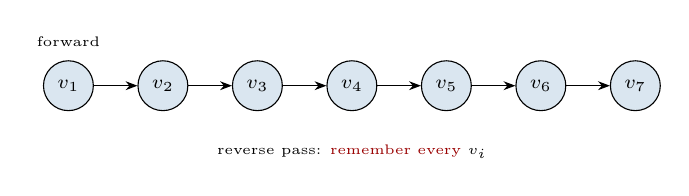
\begin{tikzpicture}[node distance=6mm, every node/.style={font=\scriptsize}]
\foreach \i in {1,...,7} {\node[draw, circle, fill=softblue!20, minimum size=5mm] (v\i) at (\i*1.2,0) {$v_{\i}$};}
\foreach \i in {1,...,6} {\pgfmathtruncatemacro{\j}{\i+1}\draw[-{Stealth[length=1.5mm]}] (v\i) -- (v\j);}
\node[above=0.5mm of v1, font=\tiny] {forward};
\node[below=3mm of v4, font=\tiny, align=center] {reverse pass: \emphc{remember every} $v_i$};
\end{tikzpicture}
\end{center}
\textbf{When this bites.}
\begin{itemize}\itemsep1pt
\item 10\,000-step trajectory with back-prop through all of it: memory $\propto T\times(\text{state dim})$; OOM on a laptop.
\item PINN training with deep nets and many collocation points: tens of millions of graph nodes.
\end{itemize}
\textbf{Mitigations.}
\begin{itemize}\itemsep1pt
\item \emphc{Path averaging / mini-batching} over trajectory segments (notebook~02).
\item \emphc{Gradient checkpointing}: recompute parts of the graph on the way back (\texttt{tf.recompute\_grad}).
\item \emphc{Truncated back-prop-through-time} for long recurrences.
\item \emphc{Forward mode} when $\#\text{inputs}$ is small.
\end{itemize}
\end{frame}

\begin{frame}{Pitfall 4: no structural insight}
\small AD returns \emph{a number}, not an \emph{expression}. Whenever the expression is worth seeing, AD hides it.
\vspace{4pt}
\begin{columns}[t]
\column{0.5\textwidth}
\textbf{Examples of useful structure}
\begin{itemize}\itemsep2pt
\item \emphc{Cancellations}: $u'(C_t) - \beta u'(C_{t+1})\,r$ has the same sign structure as the gross growth rate -- obvious from the formula, invisible in a number.
\item \emphc{Monotonicity}: $V'(K) > 0$ is an inequality you can often read off $\partial \mathcal{L}/\partial K$.
\item \emphc{Scaling laws}: $\partial V/\partial A$ for TFP $A$ is linear in $A$ -- useful for normalization.
\item \emphc{Sufficient statistics}: derivative is only a function of certain summaries.
\end{itemize}
\column{0.5\textwidth}
\textbf{Practical advice}
\begin{itemize}\itemsep2pt
\item Do the hand derivation \emph{once} on a toy version, so you \emph{know} what the gradient should look like.
\item Cross-check on a simple case: the autodiff number should agree with the closed-form formula to machine precision (this is exactly what notebooks~03 and~04 do).
\item Use AD to scale, not to replace, economic understanding.
\end{itemize}
\end{columns}
\end{frame}

\begin{frame}[fragile]{Pitfall 5: \texttt{stop\_gradient} and the envelope theorem}
\small The envelope formula $V'(K) = \partial_1 \Pi(K, g(K))$ is only valid \emph{at the optimum}. What if we are \emph{not yet} at the optimum, i.e.\ during training?
\vspace{4pt}
\textbf{Two natural ways to code it, with different results off the optimum:}
\begin{enumerate}\itemsep3pt
\item \emphc{Treat $K' = g(K)$ as a fixed function of $K$} (i.e.\ differentiate through the policy). This gives the \emph{total} derivative, not the envelope; only correct when FOC is satisfied.
\item \emphc{Treat $K'$ as an \texttt{tf.stop\_gradient} input} (i.e.\ do \emph{not} differentiate through the policy). This gives the \emph{envelope} value directly -- the formula we derived.
\end{enumerate}
\vspace{4pt}
\textbf{At the optimum both coincide.} During training they differ; the second one is the one the hand derivation gives.
\begin{exampleblock}{What the notebooks do}
\small In notebooks~03 and~04 we \emph{compute gradients of $\Pi$ at values $K_{t+1}, K_{t+2}$ that are produced by the policy}. We do \emph{not} then additionally differentiate with respect to how the policy depends on $K_t$. Check: open the notebook and notice there is only one \texttt{GradientTape} per term, watching the \emph{variable} we differentiate with respect to. That is the \texttt{stop\_gradient} behavior, built in.
\end{exampleblock}
\end{frame}

\begin{frame}[fragile]{Pitfalls: quick reference}
\footnotesize
\begin{center}
\renewcommand{\arraystretch}{1.2}
\begin{tabular}{p{3.2cm} p{4.4cm} p{4.6cm}}
\toprule
\textbf{Pitfall} & \textbf{Symptom} & \textbf{Remedy} \\
\midrule
Kinks (ReLU, abs, max) & gradient $=0$ or undefined at the kink & smooth (softplus, FB), add noise \\
Boundary singularities & NaNs, exploding gradients & reparameterise domain; stable primitives \\
Reverse-mode memory & OOM on long graphs & checkpointing, truncated BPTT, forward mode \\
Loss of insight & hard to debug unexpected gradients & hand derivation on a toy; cross-checks \\
Envelope vs total grad & wrong loss off the optimum & differentiate w.r.t.\ the right variable; \texttt{stop\_gradient} \\
\bottomrule
\end{tabular}
\end{center}
\vspace{6pt}
\centerline{\emphc{Autodiff replaces calculus. It does \emph{not} replace thinking about the model.}}
\end{frame}

% ============================================================================
% PART 8: TAKEAWAYS
% ============================================================================

\section*{8. Takeaways}

\begin{frame}{One slide to remember}
\small
\begin{block}{The autodiff pattern for any recursive model}
\[
\boxed{\;\Pi(\text{state},\;\text{choice}) \;\;\text{written once} \;\; \Longrightarrow \;\; \partial_2 \Pi + \beta\, \mathbb{E}\bigl[\partial_1 \Pi\bigr] = 0.\;}
\]
\end{block}
\vspace{4pt}
\begin{itemize}\itemsep3pt
\item \textbf{Symbolic / FD / AD} all compute derivatives; only AD is exact, dimension-free, and works on code.
\item \textbf{Forward vs reverse mode} is a choice of traversal direction on the computational graph. Reverse is the right default for DEQNs and neural networks.
\item \textbf{The Lagrangian, the FOC, and the envelope theorem} of Brock--Mirman are all gradients of a single period payoff $\Pi$. Writing $\Pi$ once removes all of them from the coding path.
\item \textbf{Pitfalls} (kinks, singularities, memory, stop-gradient) are real but small if you know they exist.
\end{itemize}
\vspace{4pt}
\centerline{\emphc{From now on, every model in this course ships with an autodiff loss.}}
\end{frame}

\begin{frame}[fragile]{Where to go next}
\footnotesize
\begin{block}{Run the notebooks}
\begin{itemize}\itemsep1pt
\item \texttt{01\_AutoDiff\_Analytical\_Examples}: warm-ups + 2-D gradient fields from \S 4.
\item \texttt{02\_Brock\_Mirman\_AutoDiff\_DEQN}: deterministic Brock--Mirman.
\item \texttt{03\_Brock\_Mirman\_Uncertainty\_AutoDiff\_DEQN}: stochastic Brock--Mirman + Gauss--Hermite.
\item \texttt{04\_IRBC\_AutoDiff\_DEQN} (\emph{further example, self-study}): IRBC under the autodiff template -- multi-country planner Lagrangian, machine-precision cross-check vs Lecture 11 nb 01.
\end{itemize}
All include cross-checks vs hand-derived loss and vs analytical solutions.
\end{block}
\begin{block}{Further reading}
\begin{itemize}\itemsep1pt
\item Baydin, Pearlmutter, Radul \& Siskind (2018), ``Automatic differentiation in machine learning: a survey'', \emph{JMLR} 18(153). Canonical overview.
\item Griewank \& Walther (2008), \emph{Evaluating Derivatives} (SIAM). Textbook.
\item JAX autodiff cookbook: \url{https://jax.readthedocs.io/en/latest/notebooks/autodiff_cookbook.html}.
\end{itemize}
\end{block}
\centerline{Questions?}
\end{frame}

\end{document}
